\documentclass{report}

%%%%%%%%%%%%%%%%%%%%%%%% Importation de paquets %%%%%%%%%%%%%%%%%%%%
\usepackage{polyglossia}
\usepackage{graphics}
\usepackage{fontspec}
\usepackage{fancyhdr}
\usepackage{listings}
\usepackage{graphics}
\usepackage{fancyhdr}
\usepackage{vmargin}
\usepackage{epsfig}   
\usepackage{multicol}
\usepackage{multirow}



%%%%%%%%%%%%%%%%%%%%%%%% Format, langue, marges %%%%%%%%%%%%%%%%%%%%%%%%%%

\setdefaultlanguage{english}
\defaultfontfeatures{Mapping=tex-text,Scale=MatchLowercase}
\setmainfont{Linux Libertine O}
\setpapersize{A4}
\setmarginsrb   
{35mm}  % leftmargin
{20mm}  % topmargin
{35mm}  % rightmargin
{40mm}  % bottommargin
{14pt}  % headheight
{15mm}   % headsep
{20pt}  % footheight
{20mm}  % footskip

%%%%%%%%%%%%%%%%%%%%%%%% En-tete et pied de page %%%%%%%%%%%%%%%%%%%%%%%%%%
\pagestyle{fancy}
\fancyhf{}
\lhead{\scalebox{0.1}[0.1]{
\includegraphics{./Images/enseeiht}}}
\rhead{\scalebox{0.1}[0.1]{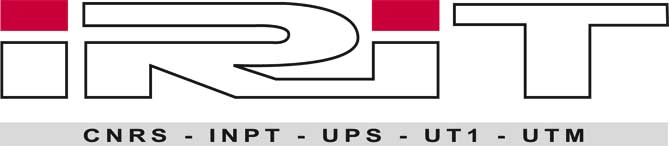
\includegraphics{./Images/irit}}
\lfoot{Three-dimensional modeling and printing}}
\rfoot{\bfseries \thepage}

\begin{document}

\bigskip
\bigskip
\bigskip
\bigskip
\bigskip
\bigskip
\bigskip
\bigskip

\begin{center}
\Huge{Project report : three-dimensional modeling and printing\\}
\bigskip
\bigskip
\Large{from January 23 to March 16, 2012}
\end{center}

\bigskip
\bigskip

\begin{center}
\large{
\textit{Vincent \textsc{Duvert} \\
Antoine \textsc{Lubineau} \\
Caroline \textsc{Naud} \\
James \textsc{Packer} \\
Florian \textsc{Ribon}} \\
\bigskip
INP-ENSEEIHT/IMA 
}
\end{center}

\bigskip
\bigskip

	This report summarizes the context, organization, work and outcomes within the project 3D modeling and printing project suggested by the VORTEX team of IRIT to some of the third-year students in the IMA department of ENSEEIHT.

\bigskip
\bigskip

\begin{figure}[!h]
\begin{center}
\scalebox{0.4}[0.4]{
\includegraphics{./Images/enseeiht}}
\end{center}
\end{figure}

\bigskip

\begin{center}
http://www.enseeiht.fr/fr/index.html \\
2 Rue Charles Camichel \\
31 071 TOULOUSE
\end{center}

\bigskip

\begin{figure}[!h]
\begin{center}
\scalebox{0.4}[0.4]{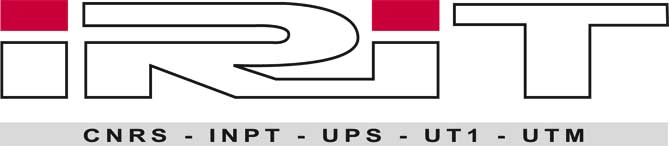
\includegraphics{./Images/irit}}
\end{center}
\end{figure}

\begin{center}
http://www.info@irit.fr\\
Université Paul Sabatier \\
118 Route de Narbonne \\
F-31062 TOULOUSE CEDEX 9
\end{center}

\thispagestyle{empty}

\newpage

\chapter*{Acknowledgments}
\addcontentsline{toc}{chapter}{\numberline{}Acknowledgments}

	Our most sincere thanks go to our technical supervisor, Lionel \textsc{Cremel} for guiding us throughout this two-month project and having initiated us in a a progressive and efficient way to the art that is project management. Our project would certainly not have got the sames results without him.\\

\bigskip

	Therefore we want to thank Axel \textsc{Carlier}, Jean \textsc{Conter} and Géraldine \textsc{Morin} for proposing such an interesting subject and for all the help and the pieces of advice they have been giving us during the project.\\

\bigskip

	We also thank all the people we have met during our visits to the manufacturing laboratory \textsc{Artilect} whogot interested in our project and agreed to share with us their expertise in this area.

\tableofcontents

\chapter{Presentation of the project}

\section{The context}

	The \textit{3D printing} phrase is used to describe the process of creating three dimensional objects from digital file using a materials printer, in a manner similar to printing images on paper. The term is most closely associated with additive manufacturing technology, where an object is created by laying down successive layers of material.\\

	Since 2003 there has been a large growth in the sale of 3D printers since the technology actually finds use in more and more fields such as the fields of jewelry, footwear, industrial design, architecture, engineering and construction (AEC), automotive, aerospace, dental and medical industries, education, geographic information systems, civil engineering, and many others.\\

	The VORTEX team (Visual Objects : from Reality To EXpression) from IRIT (Institut de Recherche en Informatique de Toulouse) is part of the numerous people having found interest in this technology and recently acquired an Ultimaker 3D printer on which she has no control over yet and that she would like to to be able to use in order to print 3D mono-color objects. To that end, she would need to be able to create, model and edit these objects within a software (to be conceived or modified) using, if possible, the multitouch screen she already owns (Acer T231H).\\

\section{The final users of the product}

	The primary final users of the product of the 3D modelling software and of the printer would be the researchers of the team of IRIT. However, they really aimed at offering this service to artists, such as those already using an Ultimaker 3D printer in the Fablab in Toulouse.

\section{The work required}

	The project was divided into two major parts. The first consisted in developing an open-source software with graphical interface that could allow to model and deform virtual 3D objects, preferably using a dualtouch screen. The second part concerned the export of this object (as a mesh) to the printer to finally print it as realistically as possible.

\section{Available resources}

\subsection{The project team}

	Our team was composed by five students from the Computing and Applied Mathematics department of ENSEEIHT who all showed a real interest in the subject. These people are listed here :

\begin{itemize}
\item Caroline \textsc{NAUD} : project manager
\item Vincent \textsc{DUVERT}
\item Antoine \textsc{LUBINEAU}
\item James \textsc{PACKER}
\item Florian \textsc{RIBON}
\end{itemize}

\subsection{Material resources}

	We list below all the material ressources that were available to us during the project :

\begin{itemize}
\item the room F117 in building F at ENSEEIHT (same building tha the one The \textsc{VORTEX} team works in
\item an Ultimaker 3D printer with a roll of PLA plastic
\item a computer with a dual-touch screen Acer T231H
\item all computer rooms of ENSEEIHT
\item our personal computers
\end{itemize}

\chapter{Project management}

\section{Project supervision}

	During the first week of the project we were introduced to Lionel \textsc{Cremel}, project manager at \textsc{Airbus}, who had volunteered to guide us in managing our project.

\section{Resource management and planning}

\section{The risk assessment}

\chapter{The specification phase}

\section{The establishment of the Statement Of Work}

\section{The redaction of the technical specifications}

\section{The general architecture of the project}

\section{The technical choices}

\chapter{The implementation phase}

\chapter{The printer calibration}

\chapter{The validation phase}

\section{Unit tests}

\section{Integration tests}

\section{Functional tests}

\section{User tests}

\addcontentsline{toc}{chapter}{\numberline{}Bibliography}

\appendix

\end{document}
